\documentclass{imanum}
\usepackage{graphicx}

\jno{drnxxx}
\received{2018}
\revised{2018}
%\accepted{3 October 2008}

\begin{document}

\title{Link prediction using effective transition}
% Short title for running heads:
\shorttitle{Link prediction using effective transition}

\author{%
{\sc
Bryn Balls-Barker\thanks{Corresponding author. Email: bryn@mathematics.byu.edu},
Ben Webb\thanks{Email: bwebb@mathematics.byu.edu}
} \\[2pt]
Department of Mathematics, Brigham Young University, 275 TMCB Provo, UT 84604
}
% Short list of authors for running heads:
\shortauthorlist{Balls-Barker, Webb}

\maketitle

\begin{abstract}
% Body of abstract:
{Here is my abstract.}
% Keywords:
{here are some key words.}
\end{abstract}


\section{Introduction}
\label{sec;introduction}

This is an introduction to the paper. 

Background on network theory.

Background on the link prediction problem. This includes an overview of existing techniques for link prediction and some mention of how techniques work better on certain types of graphs.

Really brief into to our new method. Mention that we will walk through the derivation and algorithm, the alternate versions, and some results.

\section{Effective Transition}
\label{sec;effectivetransition}

In this section we introduce the motivation for our new method.

Discuss the idea of effective transition and the effective transition matrix. 

Make statement about isoradial reduction. Prove this is equivalent to the effective transition.

Prove stationary probabilities for M and E(M) are the same.

Prove when isoradial reduction exists. 

\section{Algorithm for Strongly Connected Graphs}
\label{sec;strong}

Describe basic algorithm for strongly connected graphs. Should be very straight forward. 

Make a comment about directed/undirected, weighted/unweighted.

\subsection{Results}
Maybe show results using this algorithm. 

\section{Algorithm for Weakly Connected/Disconnected Graphs}
Describe issues with above algorithm if not already done.

Walk through derivation of new algorithm, and justification.

Explain how this algorithm and modification still gives effective transition.

Something along the lines of: Ignoring the other strongly connected components is fine because the probability of transitioning through them is zero.

\subsection{Results}
Maybe show results here.

Otherwise there is the option to show both the strongly and weakly connected results together in a new section below. 

\section{Approximating Effective Transition}

\subsection{Derivation}
Comment on how we can only handle smaller networks right now, we want a way to handle bigger networks.

Introduce the Approximation of Effective Transition.

Prove this approximation converges to the effective transition as computed above. 

Show something about what values of k are the best. And make a comment about what that optimal k value tells us about networks. 

\subsection{Results}
Here we have the results using the approximation for both the strongly connected and weakly connected graphs. And we make some notes about the time improvement and the accuracy change.

Probably also show results for bigger graphs that couldn't be handled before. 

\section{Additional Results}
We have mentioned before that this method can be used on all types of graphs. But we have only shown it using a normalization of an unweighted directed graph (maybe). In this section we will show results for the following types of graphs:

Undirected

Weighted

\clearpage


\subsection{Notation}
\label{sec3.1}



\subsection{The analysis}
\label{sec3.2}



\begin{theorem}
\label{theorem1}
Let $A$ and $L$ be the operators defined in (\ref{B0})
and (\ref{B1}).
\begin{NumberedListAlpha}
\item
If (\ref{A2}) and (\ref{A3}) hold then
\begin{equation*}
k(x) \in \mathrm{sp}(L^{-1}A) \quad \hbox{for all}\ x \in K,
\end{equation*}
where $K$ is the set of points defined in (\ref{new1}).
\item
In particular, if (\ref{A3}) holds and $k$ is continuous
throughout $\Omega$, i.e.,  $k \in C(\Omega)$, then
\begin{equation*}
k(x) \in \mathrm{sp}(L^{-1}A) \quad \hbox{for all}\ x \in \Omega.
\end{equation*}
\end{NumberedListAlpha}
\end{theorem}

\begin{proof}
Let $\tilde x \in K$ be arbitrary and assume that $\tilde x$ is
such that
$\tilde \lambda = k(\tilde x) \not\in \mathrm{sp}(L^{-1}A)$.

Clearly, there exists a set of functions
$\{ v_r \}_{r \in \mathbb{R}_{+}}$
satisfying\footnote{Note that no limit of $v_r$ as $r \rightarrow 0$
is needed in this proof. Only the existence of a set of functions
satisfying (\ref{C0.01}) and (\ref{C0.1}) is required.}
\begin{gather}
\mathrm{supp}(v_r) \subset \tilde x + U_r,
\label{C0.01}\\[3pt]
\parallel\! v_r \!\parallel_{H^1(\Omega)} = 1 ,
\label{C0.1}
\end{gather}
where
\begin{equation*}
U_r = \{ {\bf z} \in \mathbb{R}^n;\ |{\bf z}| \leq r \}.
\end{equation*}
Let
\begin{equation}
u_r = (\tilde \lambda I-L^{-1}A) v_r
\quad \hbox{for}\ r \in \mathbb{R}_+.
\label{C1}
\end{equation}

Since $\tilde \lambda \not \in \mathrm{sp}(L^{-1}A)$, it
follows that $(\tilde \lambda I-L^{-1}A)$ is invertible, and we
find that
\begin{equation}
\parallel\! v_r \!\parallel_{H^1(\Omega)}
=
\parallel\! (\tilde \lambda I-L^{-1}A)^{-1} u_{r}
\!\parallel_{H^1(\Omega)}
\leq \| (\tilde \lambda I-L^{-1}A)^{-1} \|
\parallel\! u_r \!\parallel_{H^1(\Omega)} .
\label{C2}
\end{equation}

By (\ref{C1}), we have
\begin{equation*}
u_r = \tilde \lambda I v_r - L^{-1} A v_r
\end{equation*}
or
\begin{equation*}
L u_r = \tilde \lambda L v_r - A v_r .
\end{equation*}
Hence it follows that
\begin{equation*}
(L u_r,u_r)_1 = \tilde \lambda (L v_r,u_r)_1 - (A v_r,u_r)_1 ,
\end{equation*}
and then, from the definition of $L$ and $A$ and
by the fact that $\mathrm{supp} (v_r) \subset \tilde x + U_r$,
we find that
\begin{equation*}
\int_{\Omega} \nabla u_r \cdot \nabla u_r \, \mathrm{d}x =
\tilde \lambda \int_{\tilde x + U_r} \nabla u_r \cdot
\nabla v_r \, \mathrm{d}x -
\int_{\tilde x + U_r} \nabla u_r \cdot (k \nabla v_r) \, \mathrm{d}x
\end{equation*}
or
\begin{equation*}
\int_{\Omega} |\nabla u_{r}|^2 \, \mathrm{d}x =
\int_{\tilde x + U_r} \nabla u_r \cdot ([\tilde \lambda-k]
\nabla v_r) \, \mathrm{d}x .
\end{equation*}
Next, by the Cauchy--Schwarz inequality, we have
\begin{equation*}
\int_{\Omega} |\nabla u_{r}|^{2} \, \mathrm{d}x \leq
\left(\int_{\Omega} |\nabla u_{r}|^{2} \, \mathrm{d}x \right)^{1/2}
\left(\int_{\tilde x + U_r} (\tilde \lambda-k)^{2}
|\nabla v_{r}|^2 \, \mathrm{d}x \right)^{1/2} ,
\end{equation*}
and, consequently,
\begin{equation}
\left( \int_{\Omega} |\nabla u_r|^{2} \,
\mathrm{d}x \right)^{1/2} \leq
\mathrm{ess} \sup_{x \in \tilde x + U_r} |\tilde \lambda - k(x)|
\parallel\! v_r \!\parallel_{H^1(\Omega)}
= \mathrm{ess} \sup_{x \in \tilde x + U_r} |k(\tilde x) - k(x)| ,
\label{C3}
\end{equation}
where the last equality follows from (\ref{C0.1}).
Since $k$ is continuous at $\tilde x$, it follows that
\begin{equation*}
\lim_{r \rightarrow 0} \mathrm{ess}
\sup_{x \in \tilde x + U_r} |k(\tilde x) - k(x)| = 0.
\end{equation*}
From (\ref{C3}) and Poincar\'e's inequality we thus conclude that
there exists a constant $r^\ast \in \mathbb{R}_+$ such that
\begin{equation}
\parallel\! u_r \!\parallel_{H^1(\Omega)} <
\frac{1}{2 \| (\tilde \lambda I-L^{-1}A)^{-1} \|}
\quad \hbox{for all}\ r \in (0,r^\ast).
\label{new2}
\end{equation}

Finally, (\ref{C2}) and (\ref{new2}) imply that
\begin{equation*}
\parallel\! v_r \!\parallel_{H^1(\Omega)} < \frac{1}{2}
\quad \hbox{for all}\ r \in (0,r^\ast),
\end{equation*}
which is a contradiction to (\ref{C0.1}). Hence we conclude that
$k(\tilde x)$ must satisfy $k(\tilde x) \in \mathrm{sp}(L^{-1}A)$.

This completes the proof of part (a) of the theorem. Part (b) is a
trivial consequence of part (a).
\end{proof}

\begin{figure}[t!]
\centering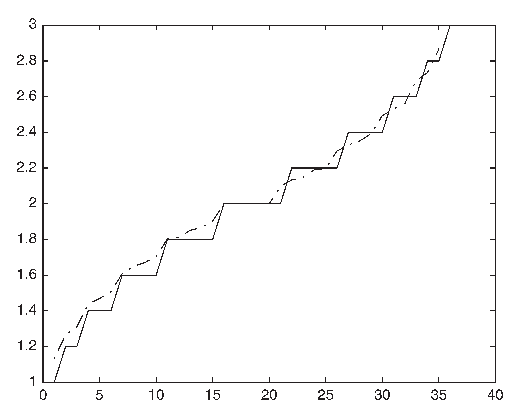
\includegraphics[scale=1.04]{fig1.eps}
\caption{Here is a caption for a picture}
\label{fig:1}
\end{figure}

\clearpage

\begin{table}[!t]
\tblcaption{Here is an example of a table}
{%
\begin{tabular}{@{}ccccc@{}}
\tblhead{$h$ & $n$ & $\max_j|\lambda_j-\mu_j|$ &
$\max_j|\lambda_j - \mu_j| / h$ & Rate}
0.2\phzzz & \phzz36 & 5.5235 & 27.6175 & -- \\
0.1\phzzz & \phz121 & 5.4286  & 54.2855 & 0.025\phz \\
0.05\phzz & \phz441 &  3.6823 & 73.6464 & 0.56\phzz \\
0.025\phz & 1681 & 2.3656 & 94.6229 & 0.6384 \\
0.0167 & 3721 & 1.1833 & 71.0001 & 1.7169 \\
0.0125 & 6561 & 0.8723 & 69.7820 & 1.0526
\lastline
\end{tabular}
}
\label{table3}
\end{table}

\end{document}
